% This LaTeX document needs to be compiled with XeLaTeX.
\documentclass[10pt]{article}
\usepackage[utf8]{inputenc}
\usepackage{graphicx}
\usepackage[export]{adjustbox}
\graphicspath{ {./images/} }
\usepackage{amsmath}
\usepackage{amsfonts}
\usepackage{amssymb}
\usepackage[version=4]{mhchem}
\usepackage{stmaryrd}
\usepackage{multirow}
\usepackage[fallback]{xeCJK}
\usepackage{polyglossia}
\usepackage{fontspec}
\setCJKmainfont{Noto Serif CJK TC}

\setmainlanguage{polish}
\setmainfont{CMU Serif}

\title{EGZAMIN MATURALNY }

\author{}
\date{}


\begin{document}
\maketitle
Arkusz zawiera informacje prawnie chronione do momentu rozpoczęcia egzaminu.

KOD\\
PESEL\\
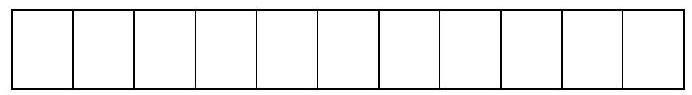
\includegraphics[max width=\textwidth, center]{2024_11_21_729eaf473b8ab3a92504g-01}\\
\(\square\)

\section*{Z MATEMATYKI}
\section*{POZIOM PODSTAWOWY}
\section*{Instrukcja dla zdającego}
\begin{enumerate}
  \item Sprawdź, czy arkusz egzaminacyjny zawiera 26 stron (zadania 1-34). Ewentualny brak zgłoś przewodniczącemu zespołu nadzorującego egzamin.
  \item Rozwiązania zadań i odpowiedzi wpisuj w miejscu na to przeznaczonym.
  \item Odpowiedzi do zadań zamkniętych (1-25) zaznacz na karcie odpowiedzi, w części karty przeznaczonej dla zdającego. Zamaluj \(\square\) pola do tego przeznaczone. Błędne zaznaczenie otocz kółkiem \({ }^{(\bigcirc)}\) zaznacz właściwe.
  \item Pamiętaj, że pominięcie argumentacji lub istotnych obliczeń w rozwiązaniu zadania otwartego (26-34) może spowodować, że za to rozwiązanie nie otrzymasz pełnej liczby punktów.
  \item Pisz czytelnie i używaj tylko długopisu lub pióra z czarnym tuszem lub atramentem.
  \item Nie używaj korektora, a błędne zapisy wyraźnie przekreśl.
  \item Pamiętaj, że zapisy w brudnopisie nie będą oceniane.
  \item Możesz korzystać z zestawu wzorów matematycznych, cyrkla i linijki oraz kalkulatora prostego.
  \item Na tej stronie oraz na karcie odpowiedzi wpisz swój numer PESEL i przyklej naklejkę z kodem.
  \item Nie wpisuj żadnych znaków w części przeznaczonej dla egzaminatora.
\end{enumerate}

UZUPELNIA ZESPÓE NADZORUJĄCY\\
Uprawnienia zdającego do:\\
\(\square\) dostosowania kryteriów ocenianianieprzenoszenia zaznaczeń na kartę\\
\(\square\) dostosowania w zw. z dyskalkulią

5 MAJA 2020

Godzina rozpoczęcia:\\
9:00

Czas pracy:\\
170 minut

\section*{Liczba punktów do uzyskania: 50}
\section*{ZADANIA ZAMKNIĘTE}
W kȧ̇dym z zadań od 1. do 25. wybierz i zaznacz na karcie odpowiedzi poprawna odpowiedź.

\section*{Zadanie 1. (1 pkt)}
Wartość wyrażenia \(x^{2}-6 x+9\) dla \(x=\sqrt{3}+3\) jest równa\\
A. 1\\
B. 3\\
C. \(1+2 \sqrt{3}\)\\
D. \(1-2 \sqrt{3}\)

\section*{Zadanie 2. (1 pkt)}
Liczba \(\frac{2^{50} \cdot 3^{40}}{36^{10}}\) jest równa\\
A. \(6^{70}\)\\
B. \(6^{45}\)\\
C. \(2^{30} \cdot 3^{20}\)\\
D. \(2^{10} \cdot 3^{20}\)

\section*{Zadanie 3. (1 pkt)}
Liczba \(\log _{5} \sqrt{125}\) jest równa\\
A. \(\frac{2}{3}\)\\
B. 2\\
C. 3\\
D. \(\frac{3}{2}\)

\section*{Zadanie 4. (1 pht)}
Cenę \(x\) pewnego towaru obniżono o \(20 \%\) i otrzymano cenę \(y\). Aby przywrócić cenę \(x\), nową cenę \(y\) należy podnieść o\\
A. \(25 \%\)\\
B. \(20 \%\)\\
C. \(15 \%\)\\
D. \(12 \%\)

\section*{Zadanie 5. (1 pkt)}
Zbiorem wszystkich rozwiązań nierówności \(3(1-x)>2(3 x-1)-12 x\) jest przedział\\
A. \(\left(-\frac{5}{3},+\infty\right)\)\\
B. \(\left(-\infty, \frac{5}{3}\right)\)\\
C. \(\left(\frac{5}{3},+\infty\right)\)\\
D. \(\left(-\infty,-\frac{5}{3}\right)\)

\section*{Zadanie 6. (1 pht)}
Suma wszystkich rozwiązań równania \(x(x-3)(x+2)=0\) jest równa\\
A. 0\\
B. 1\\
C. 2\\
D. 3

\section*{BRUDNOPIS (nie podlega ocenie)}
\begin{center}

\includegraphics[max width=\textwidth]{2024_11_21_729eaf473b8ab3a92504g-03}
\end{center}

\section*{Informacja do zadań 7.-9.}
Funkcja kwadratowa \(f\) jest określona wzorem \(f(x)=a(x-1)(x-3)\). Na rysunku przedstawiono fragment paraboli będącej wykresem tej funkcji. Wierzchołkiem tej paraboli jest punkt \(W=(2,1)\).\\
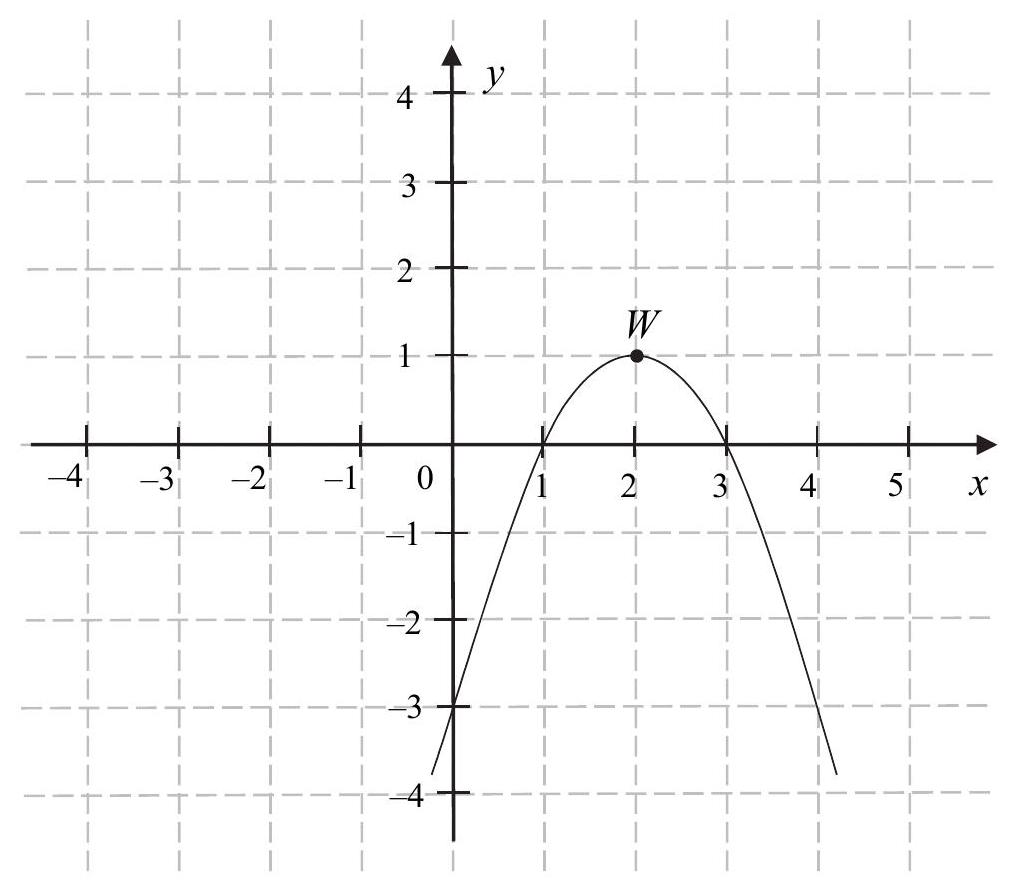
\includegraphics[max width=\textwidth, center]{2024_11_21_729eaf473b8ab3a92504g-04}

\section*{Zadanie 7. (1 pkt)}
Współczynnik \(a\) we wzorze funkcji \(f\) jest równy\\
A. 1\\
B. 2\\
C. -2\\
D. -1

\section*{Zadanie 8. (1 pkt)}
Największa wartość funkcji \(f\) w przedziale \(\langle 1,4\rangle\) jest równa\\
A. -3\\
B. 0\\
C. 1\\
D. 2

\section*{Zadanie 9. (1 pht)}
Osią symetrii paraboli będącej wykresem funkcji \(f\) jest prosta o równaniu\\
A. \(x=1\)\\
B. \(x=2\)\\
C. \(y=1\)\\
D. \(y=2\)

\section*{BRUDNOPIS (nie podlega ocenie)}
\begin{center}

\includegraphics[max width=\textwidth]{2024_11_21_729eaf473b8ab3a92504g-05}
\end{center}

\section*{Zadanie 10. (1 pkt)}
Równanie \(x(x-2)=(x-2)^{2}\) w zbiorze liczb rzeczywistych\\
A. nie ma rozwiązań.\\
B. ma dokładnie jedno rozwiązanie: \(x=2\).\\
C. ma dokładnie jedno rozwiązanie: \(x=0\).\\
D. ma dwa różne rozwiązania: \(x=1\) i \(x=2\).

\section*{Zadanie 11. (1 pkt)}
Na rysunku przedstawiono fragment wykresu funkcji liniowej \(f\) określonej wzorem \(f(x)=a x+b\).\\
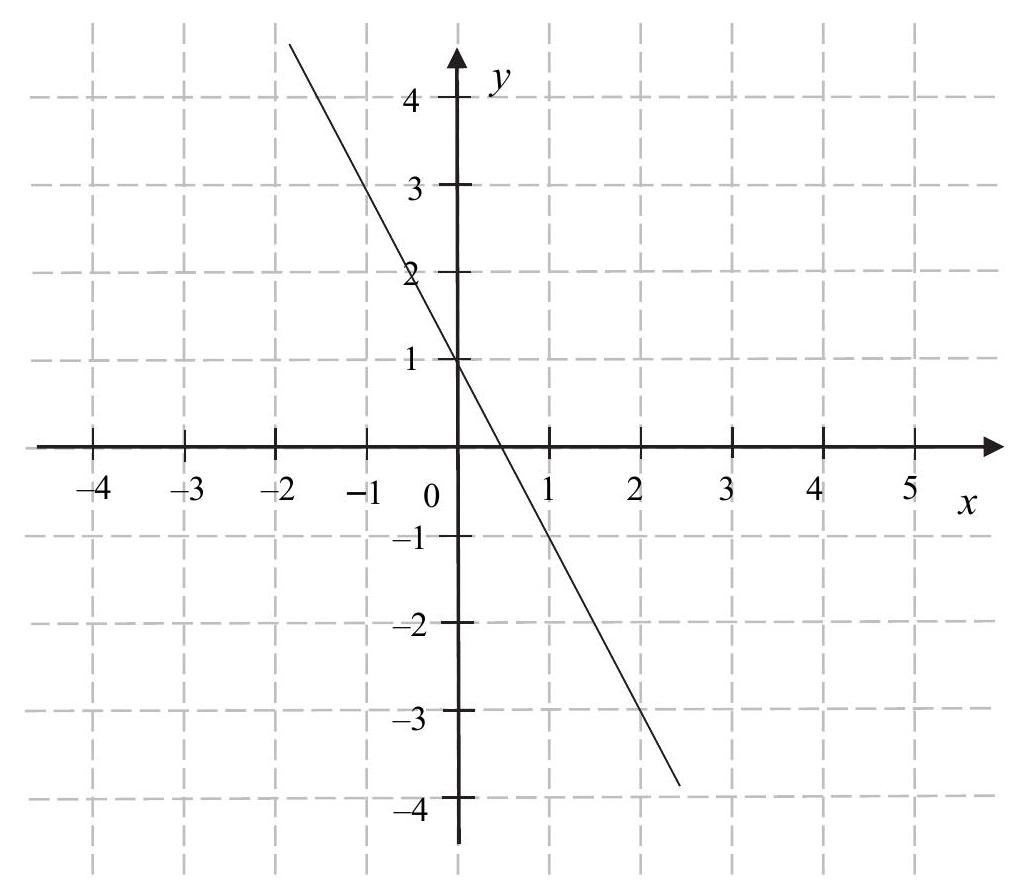
\includegraphics[max width=\textwidth, center]{2024_11_21_729eaf473b8ab3a92504g-06}

Współczynniki \(a\) oraz \(b\) we wzorze funkcji \(f\) spełniają zależność\\
A. \(a+b>0\)\\
B. \(a+b=0\)\\
C. \(a \cdot b>0\)\\
D. \(a \cdot b<0\)

\section*{Zadanie 12. (1 pkt)}
Funkcja \(f\) jest określona wzorem \(f(x)=4^{-x}+1\) dla każdej liczby rzeczywistej \(x\). Liczba \(f\left(\frac{1}{2}\right)\) jest równa\\
A. \(\frac{1}{2}\)\\
B. \(\frac{3}{2}\)\\
C. 3\\
D. 17

\section*{Zadanie 13. (1 pkt)}
Proste o równaniach \(y=(m-2) x\) oraz \(y=\frac{3}{4} x+7\) są równoległe. Wtedy\\
A. \(m=-\frac{5}{4}\)\\
B. \(m=\frac{2}{3}\)\\
C. \(m=\frac{11}{4}\)\\
D. \(m=\frac{10}{3}\)

\section*{BRUDNOPIS (nie podlega ocenie)}
\begin{center}

\includegraphics[max width=\textwidth]{2024_11_21_729eaf473b8ab3a92504g-07}
\end{center}

\section*{Zadanie 14. (1 pkt)}
Ciąg \(\left(a_{n}\right)\) jest określony wzorem \(a_{n}=2 n^{2}\) dla \(n \geq 1\). Różnica \(a_{5}-a_{4}\) jest równa\\
A. 4\\
B. 20\\
C. 36\\
D. 18

\section*{Zadanie 15. (1 pkt)}
W ciągu arytmetycznym \(\left(a_{n}\right)\), określonym dla \(n \geq 1\), czwarty wyraz jest równy 3 , a różnica tego ciągu jest równa 5. Suma \(a_{1}+a_{2}+a_{3}+a_{4}\) jest równa\\
A. -42\\
B. -36\\
C. -18\\
D. 6

\section*{Zadanie 16. (1 pkt)}
Punkt \(A=\left(\frac{1}{3},-1\right)\) należy do wykresu funkcji liniowej \(f\) określonej wzorem \(f(x)=3 x+b\). Wynika stąd, że\\
A. \(b=2\)\\
B. \(b=1\)\\
C. \(b=-1\)\\
D. \(b=-2\)

\section*{Zadanie 17. (1 pkt)}
Punkty \(A, B, C, D\) leżą na okręgu o środku w punkcie \(O\). Kąt środkowy \(D O C\) ma miarę \(118^{\circ}\) (zobacz rysunek).\\
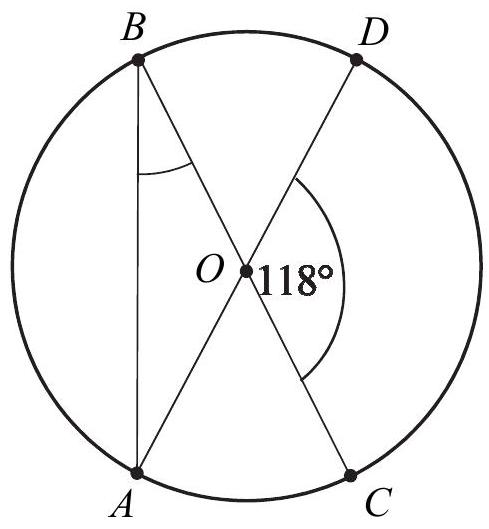
\includegraphics[max width=\textwidth, center]{2024_11_21_729eaf473b8ab3a92504g-08}

Miara kąta \(A B C\) jest równa\\
A. \(59^{\circ}\)\\
B. \(48^{\circ}\)\\
C. \(62^{\circ}\)\\
D. \(31^{\circ}\)

\section*{Zadanie 18. (1 pkt)}
Prosta przechodząca przez punkty \(A=(3,-2)\) i \(B=(-1,6)\) jest określona równaniem\\
A. \(y=-2 x+4\)\\
B. \(y=-2 x-8\)\\
C. \(y=2 x+8\)\\
D. \(y=2 x-4\)

\section*{BRUDNOPIS (nie podlega ocenie)}
\begin{center}

\includegraphics[max width=\textwidth]{2024_11_21_729eaf473b8ab3a92504g-09}
\end{center}

\section*{Zadanie 19. (1 pkt)}
Dany jest trójkąt prostokątny o kątach ostrych \(\alpha\) i \(\beta\) (zobacz rysunek).\\
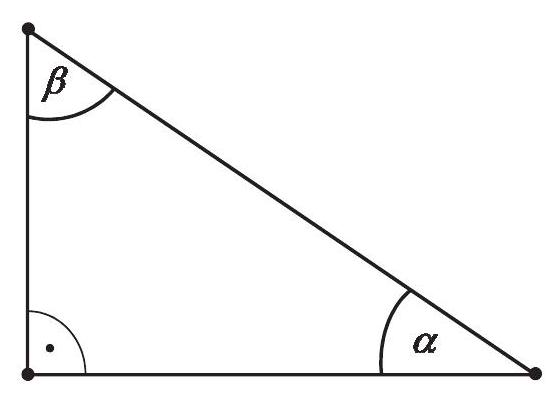
\includegraphics[max width=\textwidth, center]{2024_11_21_729eaf473b8ab3a92504g-10}

Wyrażenie \(2 \cos \alpha-\sin \beta\) jest równe\\
A. \(2 \sin \beta\)\\
B. \(\cos \alpha\)\\
C. 0\\
D. 2

\section*{Zadanie 20. (1 pkt)}
Punkt \(B\) jest obrazem punktu \(A=(-3,5)\) w symetrii względem początku układu współzzędnych. Długość odcinka \(A B\) jest równa\\
A. \(2 \sqrt{34}\)\\
B. 8\\
C. \(\sqrt{34}\)\\
D. 12

\section*{Zadanie 21. (1 pkt)}
Ile jest wszystkich dwucyfrowych liczb naturalnych utworzonych z cyfr: 1, 3, 5, 7, 9, w których cyfry się nie powtarzają?\\
A. 10\\
B. 15\\
C. 20\\
D. 25

\section*{Zadanie 22. (1 pkt)}
Pole prostokąta \(A B C D\) jest równe 90 . Na bokach \(A B\) i \(C D\) wybrano - odpowiednio - punkty \(P\) i \(R\), takie, że \(\frac{|A P|}{|P B|}=\frac{|C R|}{|R D|}=\frac{3}{2}\) (zobacz rysunek).\\
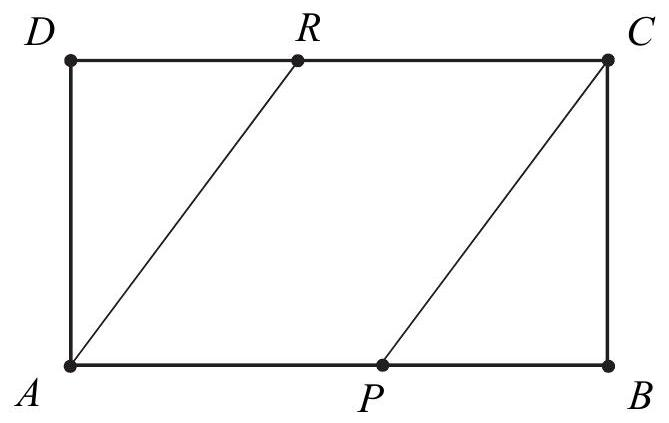
\includegraphics[max width=\textwidth, center]{2024_11_21_729eaf473b8ab3a92504g-10(1)}

Pole czworokąta \(A P C R\) jest równe\\
A. 36\\
B. 40\\
C. 54\\
D. 60

\section*{BRUDNOPIS (nie podlega ocenie)}
\begin{center}

\includegraphics[max width=\textwidth]{2024_11_21_729eaf473b8ab3a92504g-11}
\end{center}

\section*{Zadanie 23. (1 pkt)}
Cztery liczby: 2, 3, \(a, 8\), tworzące zestaw danych, są uporządkowane rosnąco. Mediana tego zestawu czterech danych jest równa medianie zestawu pięciu danych: 5, 3, 6, 8, 2. Zatem\\
A. \(a=7\)\\
B. \(a=6\)\\
C. \(a=5\)\\
D. \(a=4\)

\section*{Zadanie 24. (1 pkt)}
Dany jest sześcian \(A B C D E F G H\). Sinus kąta \(\alpha\) nachylenia przekątnej \(H B\) tego sześcianu do płaszczyzny podstawy \(A B C D\) (zobacz rysunek) jest równy\\
A. \(\frac{\sqrt{3}}{3}\)\\
B. \(\frac{\sqrt{6}}{3}\)\\
C. \(\frac{\sqrt{2}}{2}\)\\
D. \(\frac{\sqrt{6}}{2}\)\\
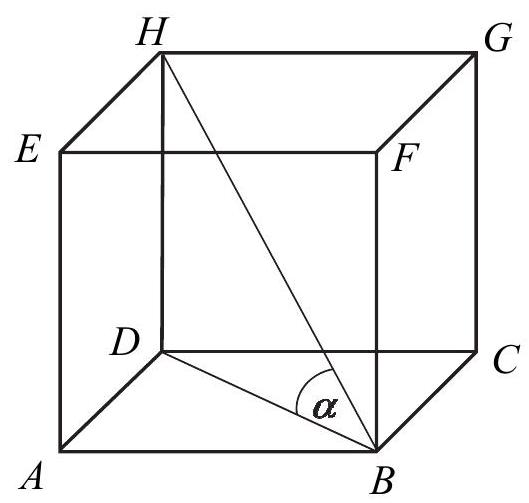
\includegraphics[max width=\textwidth, center]{2024_11_21_729eaf473b8ab3a92504g-12(1)}

\section*{Zadanie 25. (1 pkt)}
Dany jest stożek o objętości \(18 \pi\), którego przekrojem osiowym jest trójkąt \(A B C\) (zobacz rysunek).\\
Kąt CBA jest kątem nachylenia tworzącej \(l\) tego stożka do płaszczyzny jego podstawy. Tangens kąta CBA jest równy 2.\\
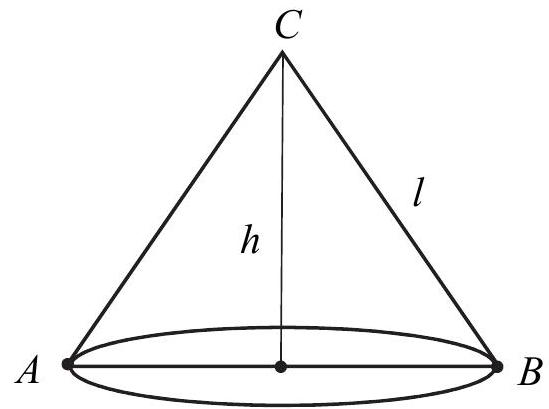
\includegraphics[max width=\textwidth, center]{2024_11_21_729eaf473b8ab3a92504g-12}

Wynika stąd, że wysokość \(h\) tego stożka jest równa\\
A. 12\\
B. 6\\
C. 4\\
D. 2

\section*{BRUDNOPIS (nie podlega ocenie)}
\begin{center}

\includegraphics[max width=\textwidth]{2024_11_21_729eaf473b8ab3a92504g-13}
\end{center}

\section*{Zadanie 26. (2 pkt)}
Rozwiąż nierówność \(2(x-1)(x+3)>x-1\).\\

\includegraphics[max width=\textwidth, center]{2024_11_21_729eaf473b8ab3a92504g-14}

Odpowiedź: \(\qquad\)

\section*{Zadanie 27. (2 pkt)}
Rozwiąż równanie \(x^{3}-9 x^{2}-4 x+36=0\).\\

\includegraphics[max width=\textwidth, center]{2024_11_21_729eaf473b8ab3a92504g-15}

Odpowiedź: \(\qquad\)

\begin{center}
\begin{tabular}{|c|l|c|c|}
\hline
\multirow{2}{*}{\begin{tabular}{l}
Wypełnia \\
egzaminator \\
\end{tabular}} & Nr zadania & 26. & 27. \\
\cline { 2 - 4 }
 & Maks. liczba pkt & 2 & 2 \\
\cline { 2 - 4 }
 & Uzyskana liczba pkt &  &  \\
\hline
\end{tabular}
\end{center}

\section*{Zadanie 28. (2 pkt)}
Wykaż, że dla każdych dwóch różnych liczb rzeczywistych \(a\) i \(b\) prawdziwa jest nierówność

\[
a(a-2 b)+2 b^{2}>0
\]

\begin{center}

\includegraphics[max width=\textwidth]{2024_11_21_729eaf473b8ab3a92504g-16}
\end{center}

\section*{Zadanie 29. (2 pkt)}
Trójkąt \(A B C\) jest równoboczny. Punkt \(E\) leży na wysokości \(C D\) tego trójkąta oraz \(|C E|=\frac{3}{4}|C D|\). Punkt \(F\) leży na boku \(B C\) i odcinek \(E F\) jest prostopadły do \(B C\) (zobacz rysunek).\\
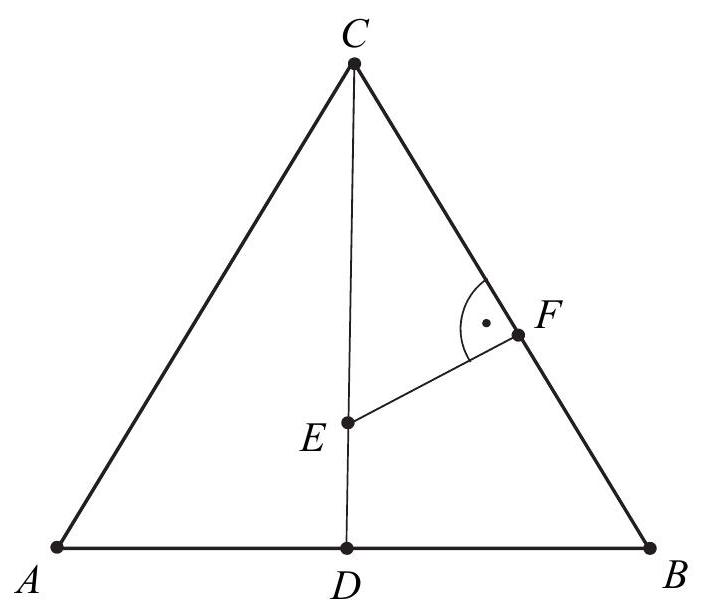
\includegraphics[max width=\textwidth, center]{2024_11_21_729eaf473b8ab3a92504g-17}

Wykaż, że \(|C F|=\frac{9}{16}|C B|\).\\

\includegraphics[max width=\textwidth, center]{2024_11_21_729eaf473b8ab3a92504g-17(1)}

\begin{center}
\begin{tabular}{|c|l|c|c|}
\hline
\multirow{2}{*}{\begin{tabular}{c}
Wypełnia \\
egzaminator \\
\end{tabular}} & Nr zadania & 28. & 29. \\
\cline { 2 - 4 }
 & Maks. liczba pkt & 2 & 2 \\
\cline { 2 - 4 }
 & Uzyskana liczba pkt &  &  \\
\hline
\end{tabular}
\end{center}

\section*{Zadanie 30. (2 pkt)}
Rzucamy dwa razy symetryczną sześcienną kostką do gry, która na każdej ściance ma inną liczbę oczek - od jednego oczka do sześciu oczek. Oblicz prawdopodobieństwo zdarzenia \(A\) polegającego na tym, że co najmniej jeden raz wypadnie ścianka z pięcioma oczkami.\\

\includegraphics[max width=\textwidth, center]{2024_11_21_729eaf473b8ab3a92504g-18}

Odpowiedź:

\section*{Zadanie 31. (2 pkt)}
Kąt \(\alpha\) jest ostry i spełnia warunek \(\frac{2 \sin \alpha+3 \cos \alpha}{\cos \alpha}=4\). Oblicz tangens kąta \(\alpha\).

\begin{center}
\begin{tabular}{|c|c|c|c|c|c|c|c|c|c|c|c|c|c|c|c|c|c|c|c|c|c|c|c|c|c|c|c|}
\hline
 &  &  &  &  &  &  &  &  &  &  &  &  &  &  &  &  &  &  &  &  &  &  &  &  &  &  &  \\
\hline
 &  &  &  &  &  &  &  &  &  &  &  &  &  &  &  &  &  &  &  &  &  &  &  &  &  &  &  \\
\hline
 &  &  &  &  &  &  &  &  &  &  &  &  &  &  &  &  &  &  &  &  &  &  &  &  &  &  &  \\
\hline
 &  &  &  &  &  &  &  &  &  &  &  &  &  &  &  &  &  &  &  &  &  &  &  &  &  &  &  \\
\hline
 &  &  &  &  &  &  &  &  &  &  &  &  &  &  &  &  &  &  &  &  &  &  &  &  &  &  &  \\
\hline
 &  &  &  &  &  &  &  &  &  &  &  &  &  &  &  &  &  &  &  &  &  &  &  &  &  &  &  \\
\hline
 &  &  &  &  &  &  &  &  &  &  &  &  &  &  &  &  &  &  &  &  &  &  &  &  &  &  &  \\
\hline
 &  &  &  &  &  &  &  &  &  &  &  &  &  &  &  &  &  &  &  &  &  &  &  &  &  &  &  \\
\hline
 &  &  &  &  &  &  &  &  &  &  &  &  &  &  &  &  &  &  &  &  &  &  &  &  &  &  &  \\
\hline
 &  &  &  &  &  &  &  &  &  &  &  &  &  &  &  &  &  &  &  &  &  &  &  &  &  &  &  \\
\hline
 &  &  &  &  &  &  &  &  &  &  &  &  &  &  &  &  &  &  &  &  &  &  &  &  &  &  &  \\
\hline
 &  &  &  &  &  &  &  &  &  &  &  &  &  &  &  &  &  &  &  &  &  &  &  &  &  &  &  \\
\hline
 &  &  &  &  &  &  &  &  &  &  &  &  &  &  &  &  &  &  &  &  &  &  &  &  &  &  &  \\
\hline
 &  &  &  &  &  &  &  &  &  &  &  &  &  &  &  &  &  &  &  &  &  &  &  &  &  &  &  \\
\hline
 &  &  &  &  &  &  &  &  &  &  &  &  &  &  &  &  &  &  &  &  &  &  &  &  &  &  &  \\
\hline
 &  &  &  &  &  &  &  &  &  &  &  &  &  &  &  &  &  &  &  &  &  &  &  &  &  &  &  \\
\hline
 &  &  &  &  &  &  &  &  &  &  &  &  &  &  &  &  &  &  &  &  &  &  &  &  &  &  &  \\
\hline
 &  &  &  &  &  &  &  &  &  &  &  &  &  &  &  &  &  &  &  &  &  &  &  &  &  &  &  \\
\hline
 &  &  &  &  &  &  &  &  &  &  &  &  &  &  &  &  &  &  &  &  &  &  &  &  &  &  &  \\
\hline
 &  &  &  &  &  &  &  &  &  &  &  &  &  &  &  &  &  &  &  &  &  &  &  &  &  &  &  \\
\hline
 &  &  &  &  &  &  &  &  &  &  &  &  &  &  &  &  &  &  &  &  &  &  &  &  &  &  &  \\
\hline
 &  &  &  &  &  &  &  &  &  &  &  &  &  &  &  &  &  &  &  &  &  &  &  &  &  &  &  \\
\hline
 &  &  &  &  &  &  &  &  &  &  &  &  &  &  &  &  &  &  &  &  &  &  &  &  &  &  &  \\
\hline
 &  &  &  &  &  &  &  &  &  &  &  &  &  &  &  &  &  &  &  &  &  &  &  &  &  &  &  \\
\hline
 &  &  &  &  &  &  &  &  &  &  &  &  &  &  &  &  &  &  &  &  &  &  &  &  &  &  &  \\
\hline
 &  &  &  &  &  &  &  &  &  &  &  &  &  &  &  &  &  &  &  &  &  &  &  &  &  &  &  \\
\hline
 &  &  &  &  &  &  &  &  &  &  &  &  &  &  &  &  &  &  &  &  &  &  &  &  &  &  &  \\
\hline
 &  &  &  &  &  &  &  &  &  &  &  &  &  &  &  &  &  &  &  &  &  &  &  &  &  &  &  \\
\hline
 &  &  &  &  &  &  &  &  &  &  &  &  &  &  &  &  &  &  &  &  &  &  &  &  &  &  &  \\
\hline
 &  &  &  &  &  &  &  &  &  &  &  &  &  &  &  &  &  &  &  &  &  &  &  &  &  &  &  \\
\hline
 &  &  &  &  &  &  &  &  &  &  &  &  &  &  &  &  &  &  &  &  &  &  &  &  &  &  &  \\
\hline
 &  &  &  &  &  &  &  &  &  &  &  &  &  &  &  &  &  &  &  &  &  &  &  &  &  &  &  \\
\hline
 &  &  &  &  &  &  &  &  &  &  &  &  &  &  &  &  &  &  &  &  &  &  &  &  &  &  &  \\
\hline
- & - &  &  &  &  &  &  &  &  &  &  &  &  &  &  &  &  &  &  &  &  &  &  &  &  &  &  \\
\hline
 & 到 &  &  &  &  &  &  &  &  &  &  &  &  &  &  &  &  &  &  &  &  &  &  &  &  &  &  \\
\hline
 &  &  &  &  &  &  &  &  &  &  &  &  &  &  &  &  &  &  &  &  &  &  &  &  &  &  &  \\
\hline
 &  &  &  &  &  &  &  &  &  &  &  &  &  &  &  &  &  &  &  &  &  &  &  &  &  &  &  \\
\hline
 &  &  &  &  &  &  &  &  &  &  &  &  &  &  &  &  &  &  &  &  &  &  &  &  &  &  &  \\
\hline
 &  &  &  &  &  &  &  &  &  &  &  &  &  &  &  &  &  &  &  &  &  &  &  &  &  &  &  \\
\hline
\end{tabular}
\end{center}

Odpowiedź: \(\qquad\)

\begin{center}
\begin{tabular}{|c|l|c|c|}
\hline
\multirow{2}{*}{\begin{tabular}{c}
Wypełnia \\
egzaminator \\
\end{tabular}} & Nr zadania & \(\mathbf{3 0 .}\) & \(\mathbf{3 1 .}\) \\
\cline { 2 - 4 }
 & Maks. liczba pkt & \(\mathbf{2}\) & \(\mathbf{2}\) \\
\cline { 2 - 4 }
 & Uzyskana liczba pkt &  &  \\
\hline
\end{tabular}
\end{center}

Strona 19 z 26

\section*{Zadanie 32. (4 pkt)}
Dany jest kwadrat \(A B C D\), w którym \(A=\left(5,-\frac{5}{3}\right)\). Przekątna \(B D\) tego kwadratu jest zawarta w prostej o równaniu \(y=\frac{4}{3} x\). Oblicz współrzędne punktu przecięcia przekątnych \(A C\) i \(B D\) oraz pole kwadratu \(A B C D\).\\

\includegraphics[max width=\textwidth, center]{2024_11_21_729eaf473b8ab3a92504g-20}\\

\includegraphics[max width=\textwidth, center]{2024_11_21_729eaf473b8ab3a92504g-21}

Odpowiedź:

\begin{center}
\begin{tabular}{|c|l|c|}
\hline
\multirow{2}{*}{\begin{tabular}{l}
Wypełnia \\
egzaminator \\
\end{tabular}} & Nr zadania & 32. \\
\cline { 2 - 3 }
 & Maks. liczba pkt & 4 \\
\cline { 2 - 3 }
 & Uzyskana liczba pkt &  \\
\hline
\end{tabular}
\end{center}

Strona 21 z 26\\
MMA\_1P

\section*{Zadanie 33. (4 pkt)}
Wszystkie wyrazy ciągu geometrycznego \(\left(a_{n}\right)\), określonego dla \(n \geq 1\), są dodatnie. Wyrazy tego ciągu spełniają warunek \(6 a_{1}-5 a_{2}+a_{3}=0\). Oblicz iloraz \(q\) tego ciągu należący do przedziału \(\langle 2 \sqrt{2}, 3 \sqrt{2}\rangle\).\\

\includegraphics[max width=\textwidth, center]{2024_11_21_729eaf473b8ab3a92504g-22}\\

\includegraphics[max width=\textwidth, center]{2024_11_21_729eaf473b8ab3a92504g-23}

Odpowiedź: \(\qquad\)

\begin{center}
\begin{tabular}{|c|l|c|}
\hline
\multirow{2}{*}{\begin{tabular}{l}
Wypelnia \\
egzaminator \\
\end{tabular}} & Nr zadania & 33. \\
\cline { 2 - 3 }
 & Maks. liczba pkt & 4 \\
\cline { 2 - 3 }
 & Uzyskana liczba pkt &  \\
\hline
\end{tabular}
\end{center}

\section*{Zadanie 34. (5 pkt)}
Dany jest ostrosłup prawidłowy czworokątny \(A B C D S\), którego krawędź boczna ma długość 6 (zobacz rysunek). Ściana boczna tego ostrosłupa jest nachylona do płaszczyzny podstawy pod kątem, którego tangens jest równy \(\sqrt{7}\). Oblicz objętość tego ostrosłupa.\\
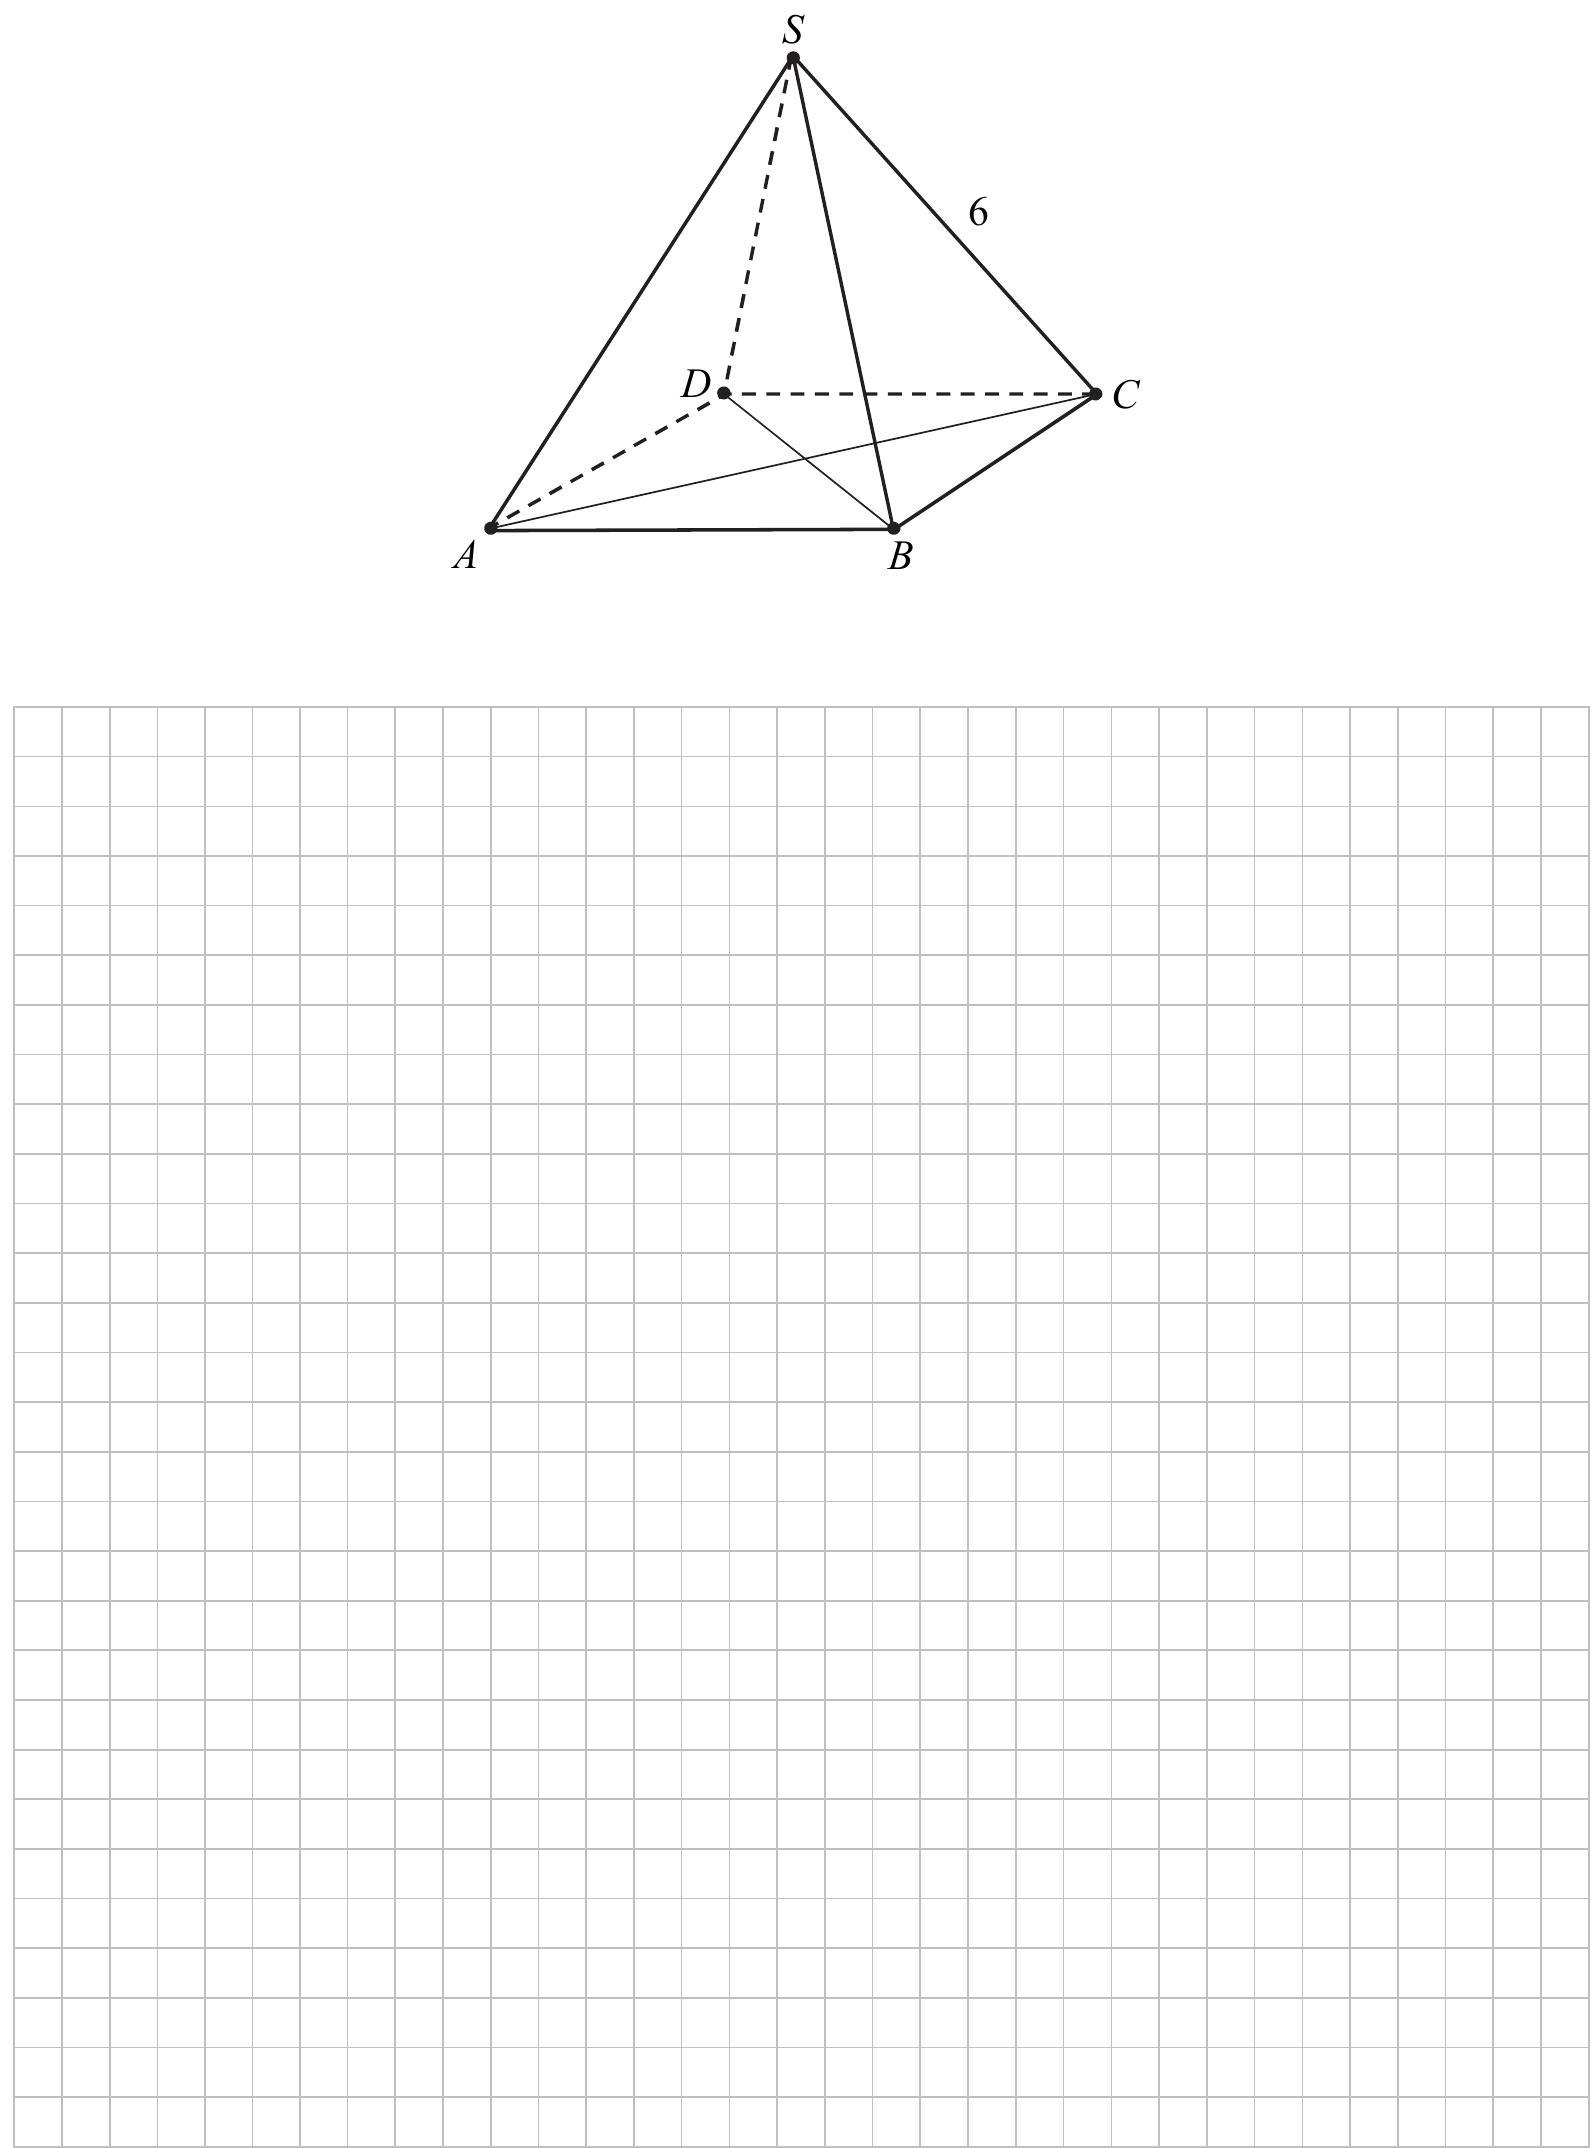
\includegraphics[max width=\textwidth, center]{2024_11_21_729eaf473b8ab3a92504g-24}\\

\includegraphics[max width=\textwidth, center]{2024_11_21_729eaf473b8ab3a92504g-25}

Odpowiedź: \(\qquad\)

\begin{center}
\begin{tabular}{|c|l|c|}
\hline
\multirow{2}{*}{\begin{tabular}{l}
Wypelnia \\
egzaminator \\
\end{tabular}} & Nr zadania & 34. \\
\cline { 2 - 3 }
 & Maks. liczba pkt & 5 \\
\cline { 2 - 3 }
 & Uzyskana liczba pkt &  \\
\hline
\end{tabular}
\end{center}

\section*{BRUDNOPIS (nie podlega ocenie)}

\end{document}